\section{実験設計}

本節では，実験目的，実験条件，実験手順について述べる．

\subsection{実験目的}
本実験は，段階的な自己開示支援が受容性の向上に与える効果を検証することを目的とする．提案手法が自己開示の深化と受容性の向上に寄与するかを明らかにするため，システムによる段階的支援の有無による比較実験を実施する．


\subsection{実験条件}

\subsubsection{実験環境}

実験はカラオケ空間をもした閉鎖的な空間で実施した．対面でのカジュアルな会話を促進するため，2つの座椅子を適度な距離を保って対面に配置し，Bluetoothスピーカーを通じて音楽を再生する．カラオケ店舗の雰囲気を模倣するため，YouTube\cite{youtube}で配信されているDAMチャンネル\cite{damchannel}の動画コンテンツを小音量で再生し，完全な無音空間を避けるようにした．また，実験室の壁面にプロジェクターでDAMチャンネルの映像を投影し，視覚的な要素も考慮した．照明は会話に支障をきたさない程度の明るさに調整することで，リラックスした雰囲気の実現を図った．

\begin{figure}[H]
    \centering
    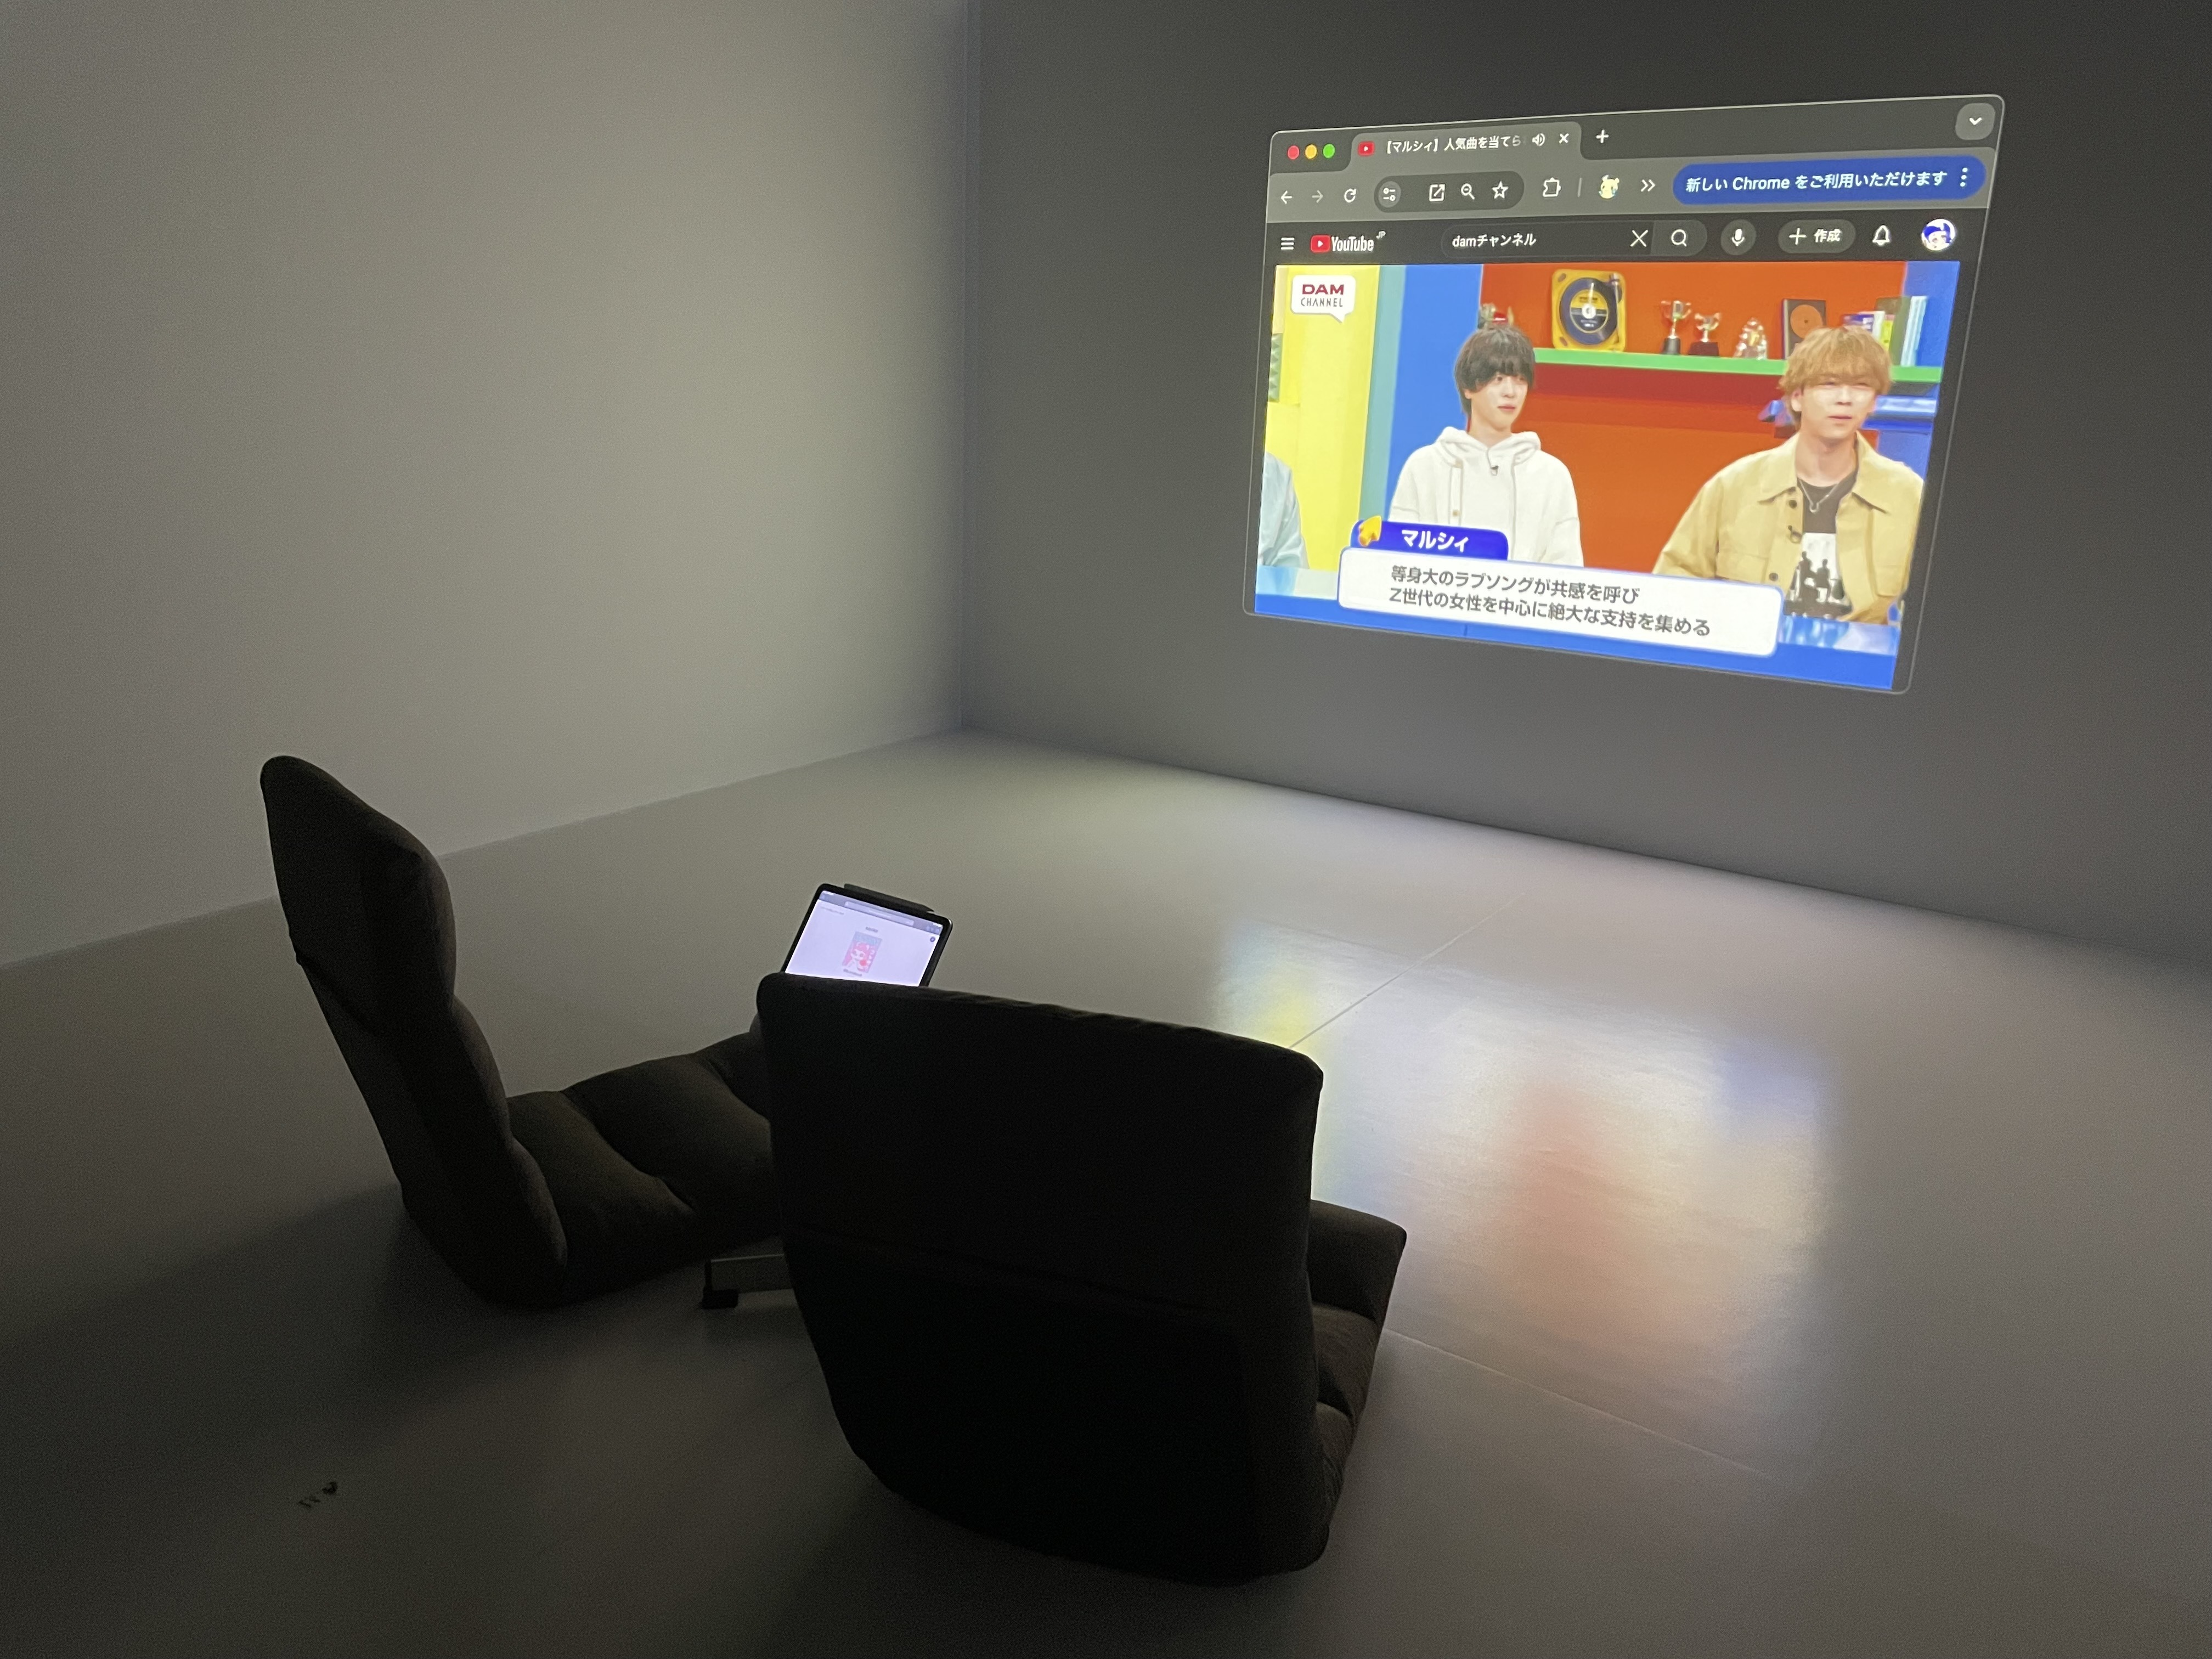
\includegraphics[width=0.75\linewidth]{image/実験環境.jpg}
    \caption{音楽共有セッションに用いる環境}
    \label{pic:実験環境}
\end{figure}


\subsubsection{実験参加者}
被験者は，年齢差がない学生・社会人の20名（18-24歳の男性8名，女性12名）を対象とし，10ペアで実験を行った．2群比較実験であるため，男女の比率が公平になるよう無作為に2群に割り当てた．

関係性は友人関係とした．友人関係とは，日常的な会話や活動を共にする程度でかつ，同じ空間で過ごしていても心理的負担を感じない関係性であり，自分の内面に関する深刻な悩み事を相談するほどの親密さには至っていない程度を対象とした．これは，初対面である場合は自己開示が重く感じられ，逆に親友レベルの関係性である場合はすでに深い自己開示を行えているため，友人という関係が最も適切であるとされている．


\subsection{実験手順}\label{実験手順}

音楽における自己開示の段階をレベル分けするため，選曲理由や楽曲にまつわる思い出の開示レベルを定義する．その後，このレベルに基づいて段階的に自己開示を促すシステムを実装する．

実験は事前準備と本実験の2段階で構成される．
事前準備では，被験者に50曲程度の「お気に入りの曲」プレイリストを作成してもらい，各楽曲に対する思い入れの強さを評価する．

本実験の音楽共有セッションでは，システムによる段階的な楽曲推薦を行う群（推薦あり群）と，支援を行わない群（推薦なし群）の2群で比較を行う．セッションは全8フェーズで構成され，各フェーズでは楽曲選択（推薦あり群はシステムが提示する候補から，推薦なし群は自身の作成したプレイリストの全楽曲から選択），楽曲再生，対話という流れで進行する．各フェーズ終了後，被験者は自己開示の度合いや楽曲体験の受容性に関する評価を行う．これらのデータを解析することで，段階的な自己開示が，相手の自己開示に対する受容性を向上させるかを検証する．

次節では，本実験で使用するシステムの設計・実装について詳しく説明する．